\subsection{Describing the System}\label{sec:sqd-mnp_setup}

\begin{figure}[ht]
    \centering
    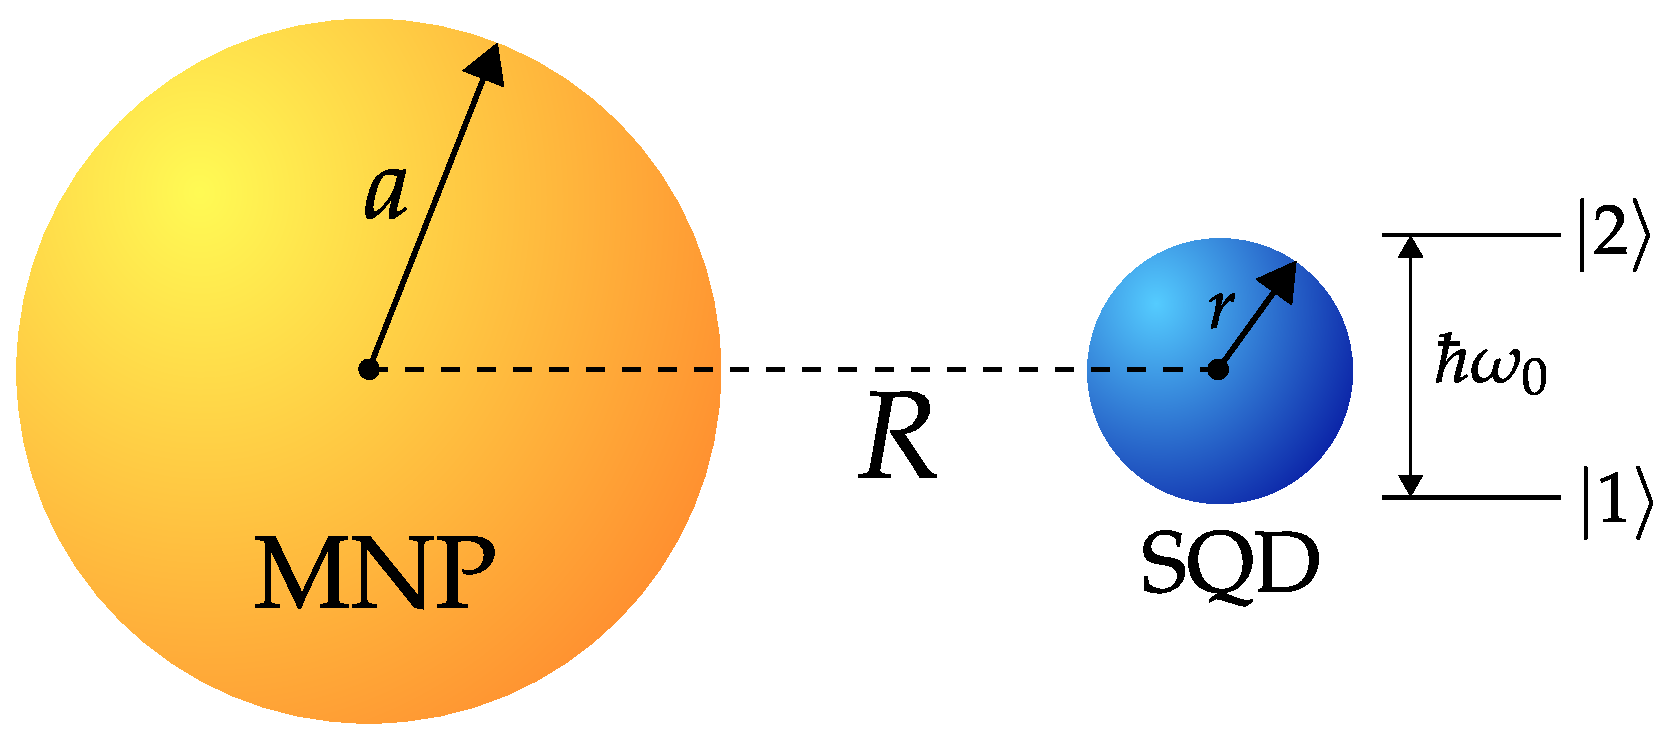
\includegraphics[width=0.8\textwidth]{sqd_mnp_schem.eps}
    \caption{Schematic diagram of a spherical metal nanoparticle (MNP) of
        radius, $a$, separated by a distance, $R$, from a spherical
        semiconducting quantum dot (SQD) of radius, $r$.  The MNP is modelled
        classically while the SQD is treated as a two-level quantum system with
        ground state, $\state{1}$, and excited state, $\state{2}$, separated by
    an energy gap of $\hbar\omega_0$.}
    \label{fig:sqd-mnp_scem}
\end{figure}

\noindent Consider a spherical, gold MNP of radius, $a$, separated by a distance,
$R$, from a spherical
SQD of radius, $r$, as shown in \cref{fig:sqd-mnp_scem}.
From \cref{eq:fields1}, when an external field $\eext(t)$ is applied, the
fields felt by the SQD and MNP are, respectively,
%
\begin{align}
    \esqd(t) &= \eext(t) + g\frac{\pmnp(t)}{\epsb R^3} \ , \label{eq:esqd}\\
    \emnp(t) &= \eext(t) + g\frac{\psqd(t)}{\epsb R^3} \ ,
\end{align}
%
where $\psqd(t)$ ($\pmnp(t)$) is the dipole moment of the SQD (MNP).
We have taken the external field to be polarized along the line connecting the
centres of the particles so that $\hat n=\hat e$. From \cref{eq:g_def}, we have
that $\vec{g}=2\hat e$ and so all fields are pointing in the direction of the
external field, $\hat e$, allowing us to drop the vector notation.

The SQD is treated as a 2-level, atomic-like system with ground state,
$\state{1}$, and excited state, $\state{2}$, separated by an energy gap of
$\hbar\omega_0$ ($\omega_0$ is known as the exciton frequency). We use the
density matrix formalism so that the SQD can be described by a $2\times
2$ density matrix, $\bm\rho(t)$, whose elements can be written as (see Appendix
REF\note{(--from differentiation)})
%
\begin{equation}
    \begin{cases}
        \dot{\Delta} &= -\frac{4\mut}{\hbar}\esqd(t)\imag{\rho_{21}} -
        \Gamma_{11}(\Delta - 1)   \\
        \dot\rho_{21} &= -\left( \Gamma_{21}+\imagn\omega_0
        \right)\rho_{21} + \imagn\frac{\mut}{\hbar}\esqd(t) \Delta
        \label{eq:eoms}
    \end{cases} \ ,
\end{equation}
%
where $\Delta(t)=\rho_{11}(t)-\rho_{22}(t)$ is the population difference between the
ground and excited states, and $\rho_{12}=\rho_{21}^*$. $\Gamma_{11}$ and $\Gamma_{21}$ are the population
decay and dephasing rates of the system respectively. The SQD is assumed to be
a
dielectric sphere with dielectric constant $\epss$ and so it has a screened
dipole matrix element,
%
\begin{equation}
    \mut=\frac{\mu_{21}}{\epseff} \ ,
\end{equation}
%
where $\mu_{21}$ is the bare
dipole matrix element and~\cite{batygin_problems_1978}
%
\begin{equation}
    \epseff=\frac{2\epsb+\epss}{3\epsb} \ .
\end{equation}
%
\note{(Not sure if these should go here or later\dots)} We take the SQD system parameters from
Ref.~\cite{zhang_semiconductor-metal_2006}, which are typical of a \ce{CdSe}
quantum dot.
The dielectric
constant is taken to be $\epss=6$ with (bare) transition dipole moment $\mu=0.65e$~nm and
exciton energy $\hbar\omega_0=2.5$~eV close to the plasmon peak of the gold MNP.
The decay and dephasing times are given by
$\Gamma_{11}^{-1}=0.8$~ns and $\Gamma_{21}^{-1}=0.3$~ns. 

The dipole moment of the SQD is
%
\begin{align}
    \psqd(t) &= \trace{\bm\rho\bm\mu} \\
    &= \mut\left( \rho_{12} + \rho_{21} \right) ,
    \label{eq:psqdt}
\end{align}
%
where $\trace{\cdots}$ is the matrix trace operator. The dipole moment of the
MNP is taken to be
%
\begin{equation}
    \pmnp(\omega) = \alphamnp(\omega)\emnp(\omega) \ ,
    \label{eq:pmnpw}
\end{equation}
%
where $\alphamnp(\omega)$ is the frequency-dependent polarizability.
For comparison with previous literature, we approximate $\alphamnp(\omega)$ by
the Clausius-Mossotti formula,
%
\begin{equation}
    \alphamnp(\omega) = a^3 \frac{\epsm(\omega)-1\epsb}{
    \epsm(\omega) + 2\epsb} \ ,
    \label{eq:alpha_mnp}
\end{equation}
%
where $\epsm(\omega)$ is the frequency-dependent dielectric function of the
bulk metal~\cite{landau_electrodynamics_1984} (we use the analytical model for
bulk gold as given by Etchegoin et al.~\cite{etchegoin_analytic_2006}).

For the external field, we shall consider the following light pulse,
%
\begin{equation}
    \eext(t) = f(t) E_0 \cos(\omega_L t) \ ,
    \label{eq:pulse_general}
\end{equation}
%
where $f(t)$ is a dimensionless pulse envelope, $\omega_L$ is the carrier (or
central) frequency and $E_0$ is the amplitude. The field strength is normally
given in terms of the intensity, $I_0$, by
%
\begin{equation}
    I_0 = \frac{c}{2}E_0^2 \ ,
    \label{eq:intensity}
\end{equation}
%
where $c$ is the speed of light. \note{$I_0=\frac{\epsilon_0 c}{2}E_0^2$, in
gaussian units, does the $\epsilon_0$ (vacuum permittivity) just disappear, or
should there be a $4\pi$ in there?\ldots}

To determine the solutions to \cref{eq:eoms}, one can (i) follow the PEOM
method in ~\cref{sec:peom}, or (ii) use analytical approximations. We shall now
describe both procedures.
